\documentclass{article}
\usepackage[hmargin=1in,vmargin=1.5in]{geometry}
\usepackage{amsmath}
\usepackage{amsfonts}
\usepackage{graphicx}
\usepackage{subcaption}
\usepackage{bm}
\newcommand{\x}{\bm x}
\title{Homework 4}
\setcounter{MaxMatrixCols}{20}
\author{Xinyi Gu, Songchen Tan}
\date{\today}
\begin{document}
\maketitle
\section{}
See the solution in Figure 1.
\begin{figure}[!ht]
    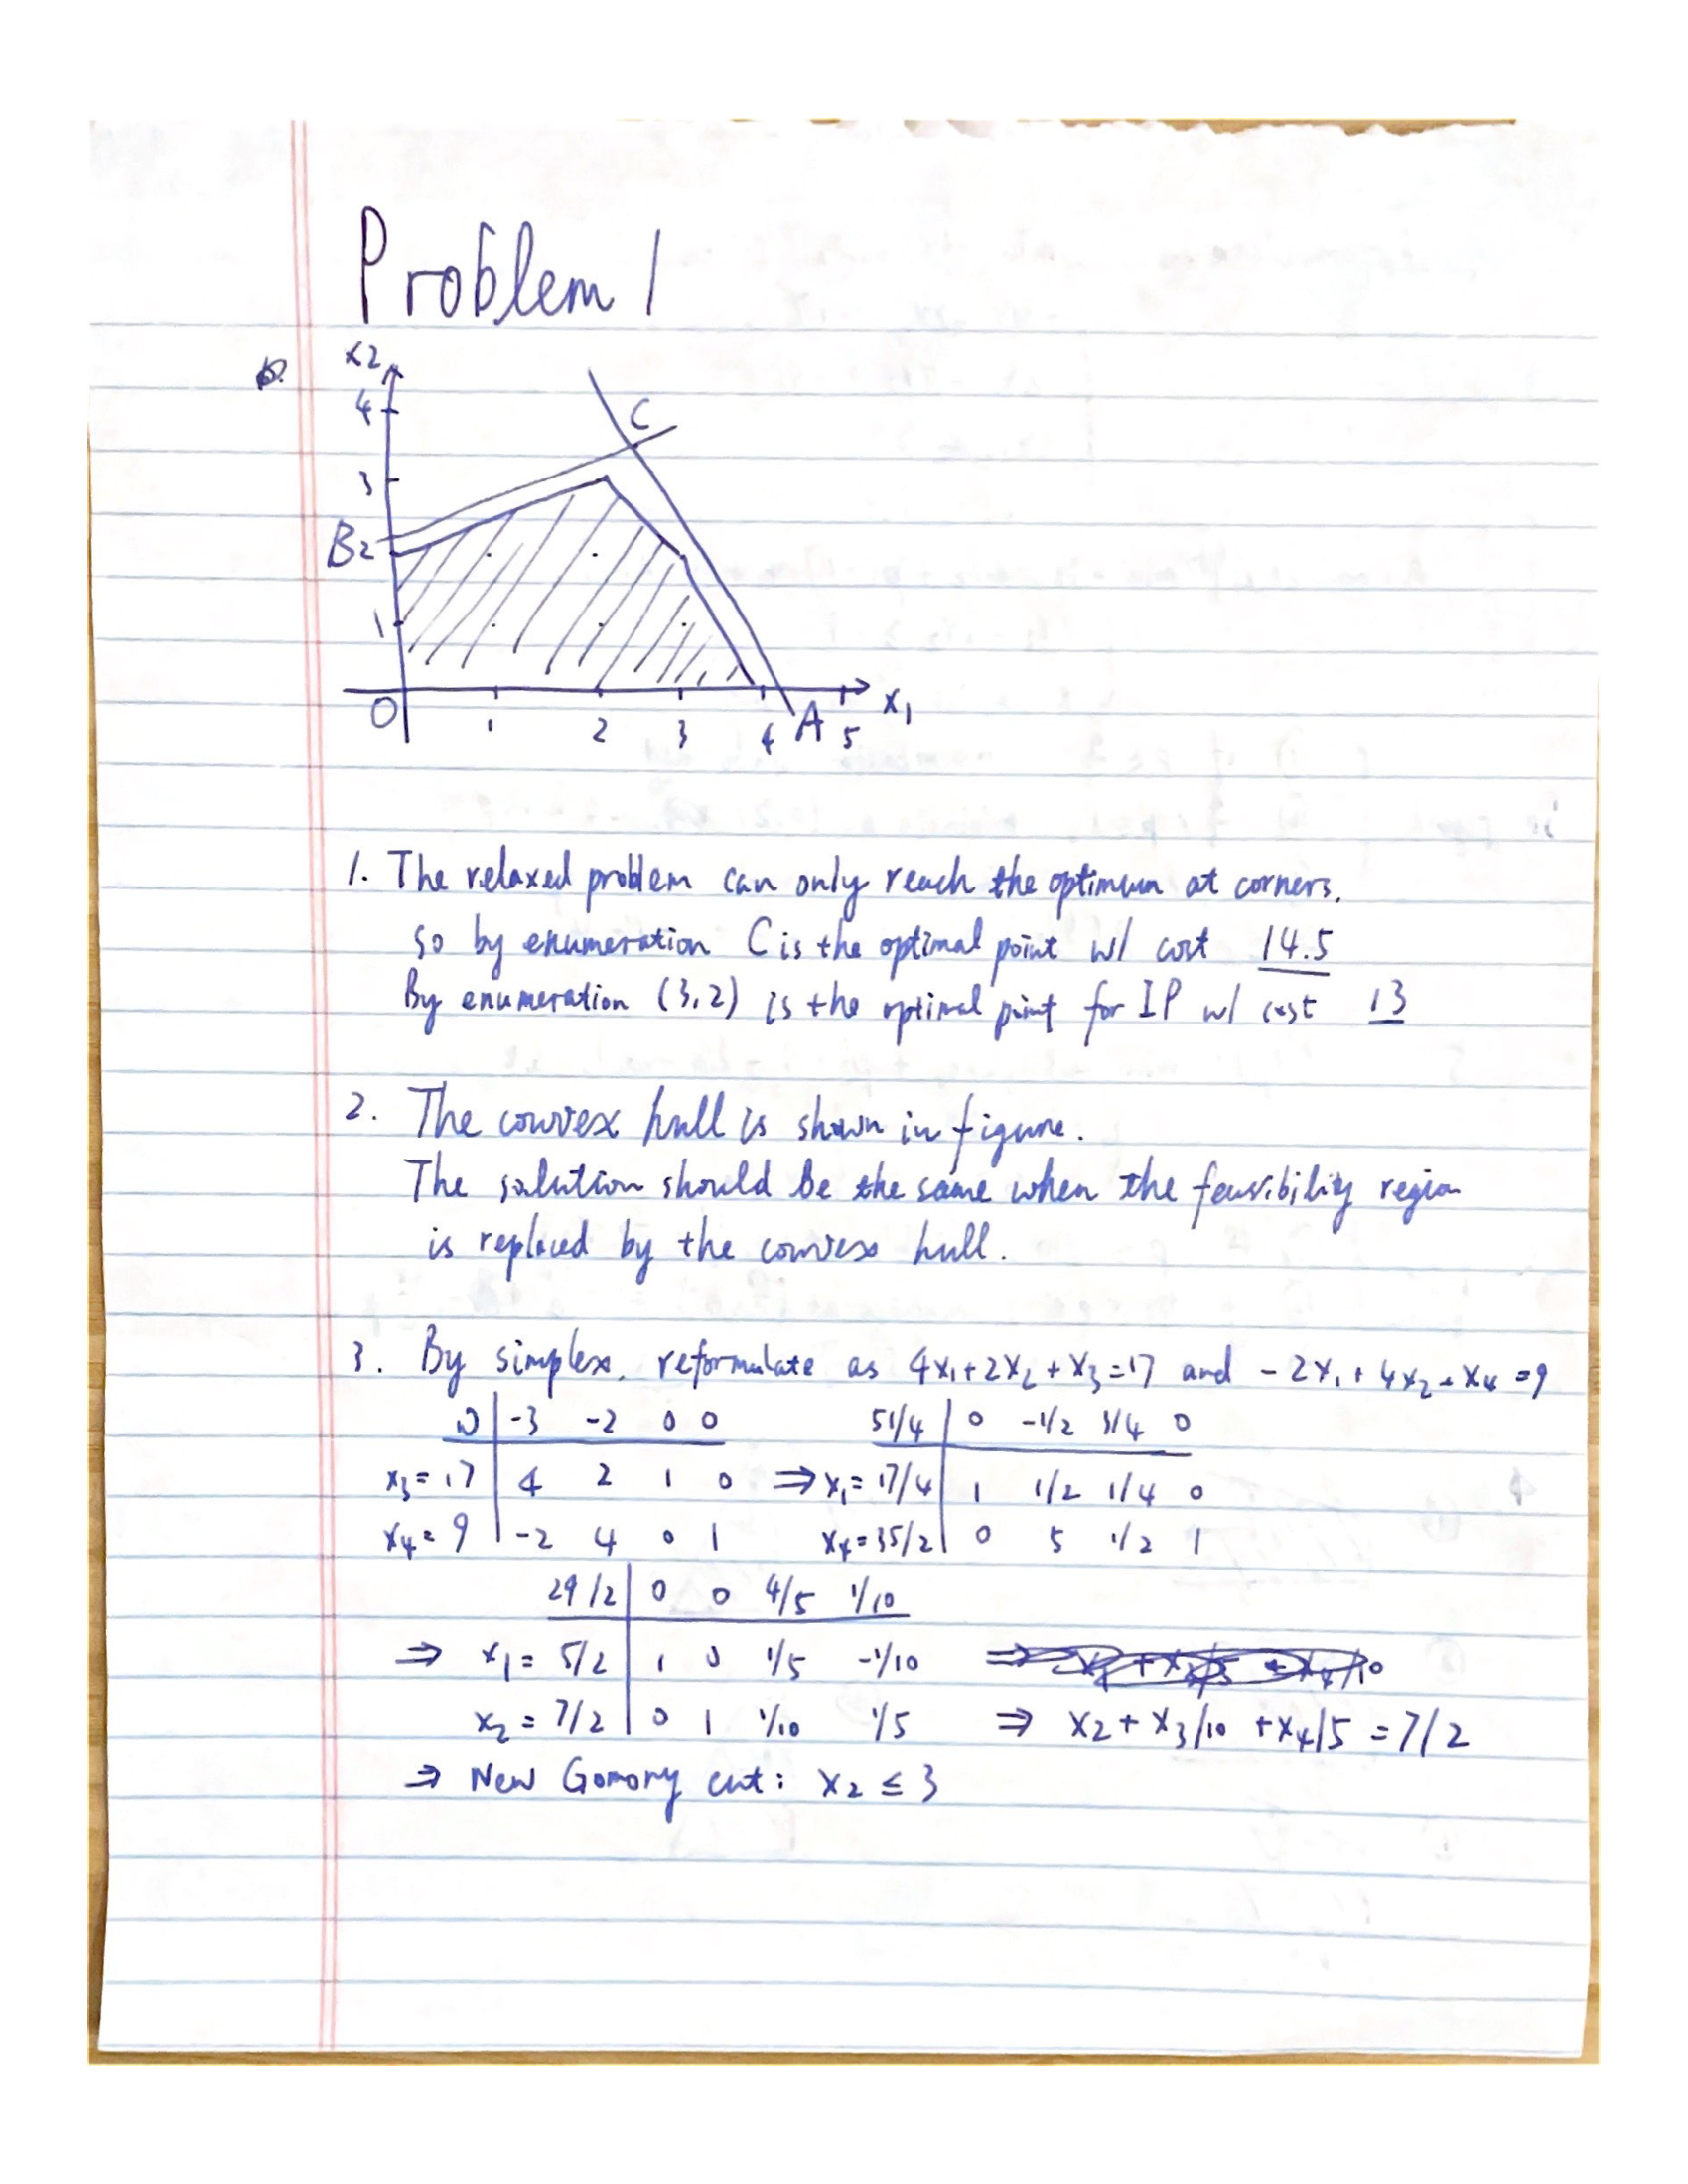
\includegraphics[width=\textwidth]{1.1.png}
\end{figure}
\begin{figure}[!ht]
    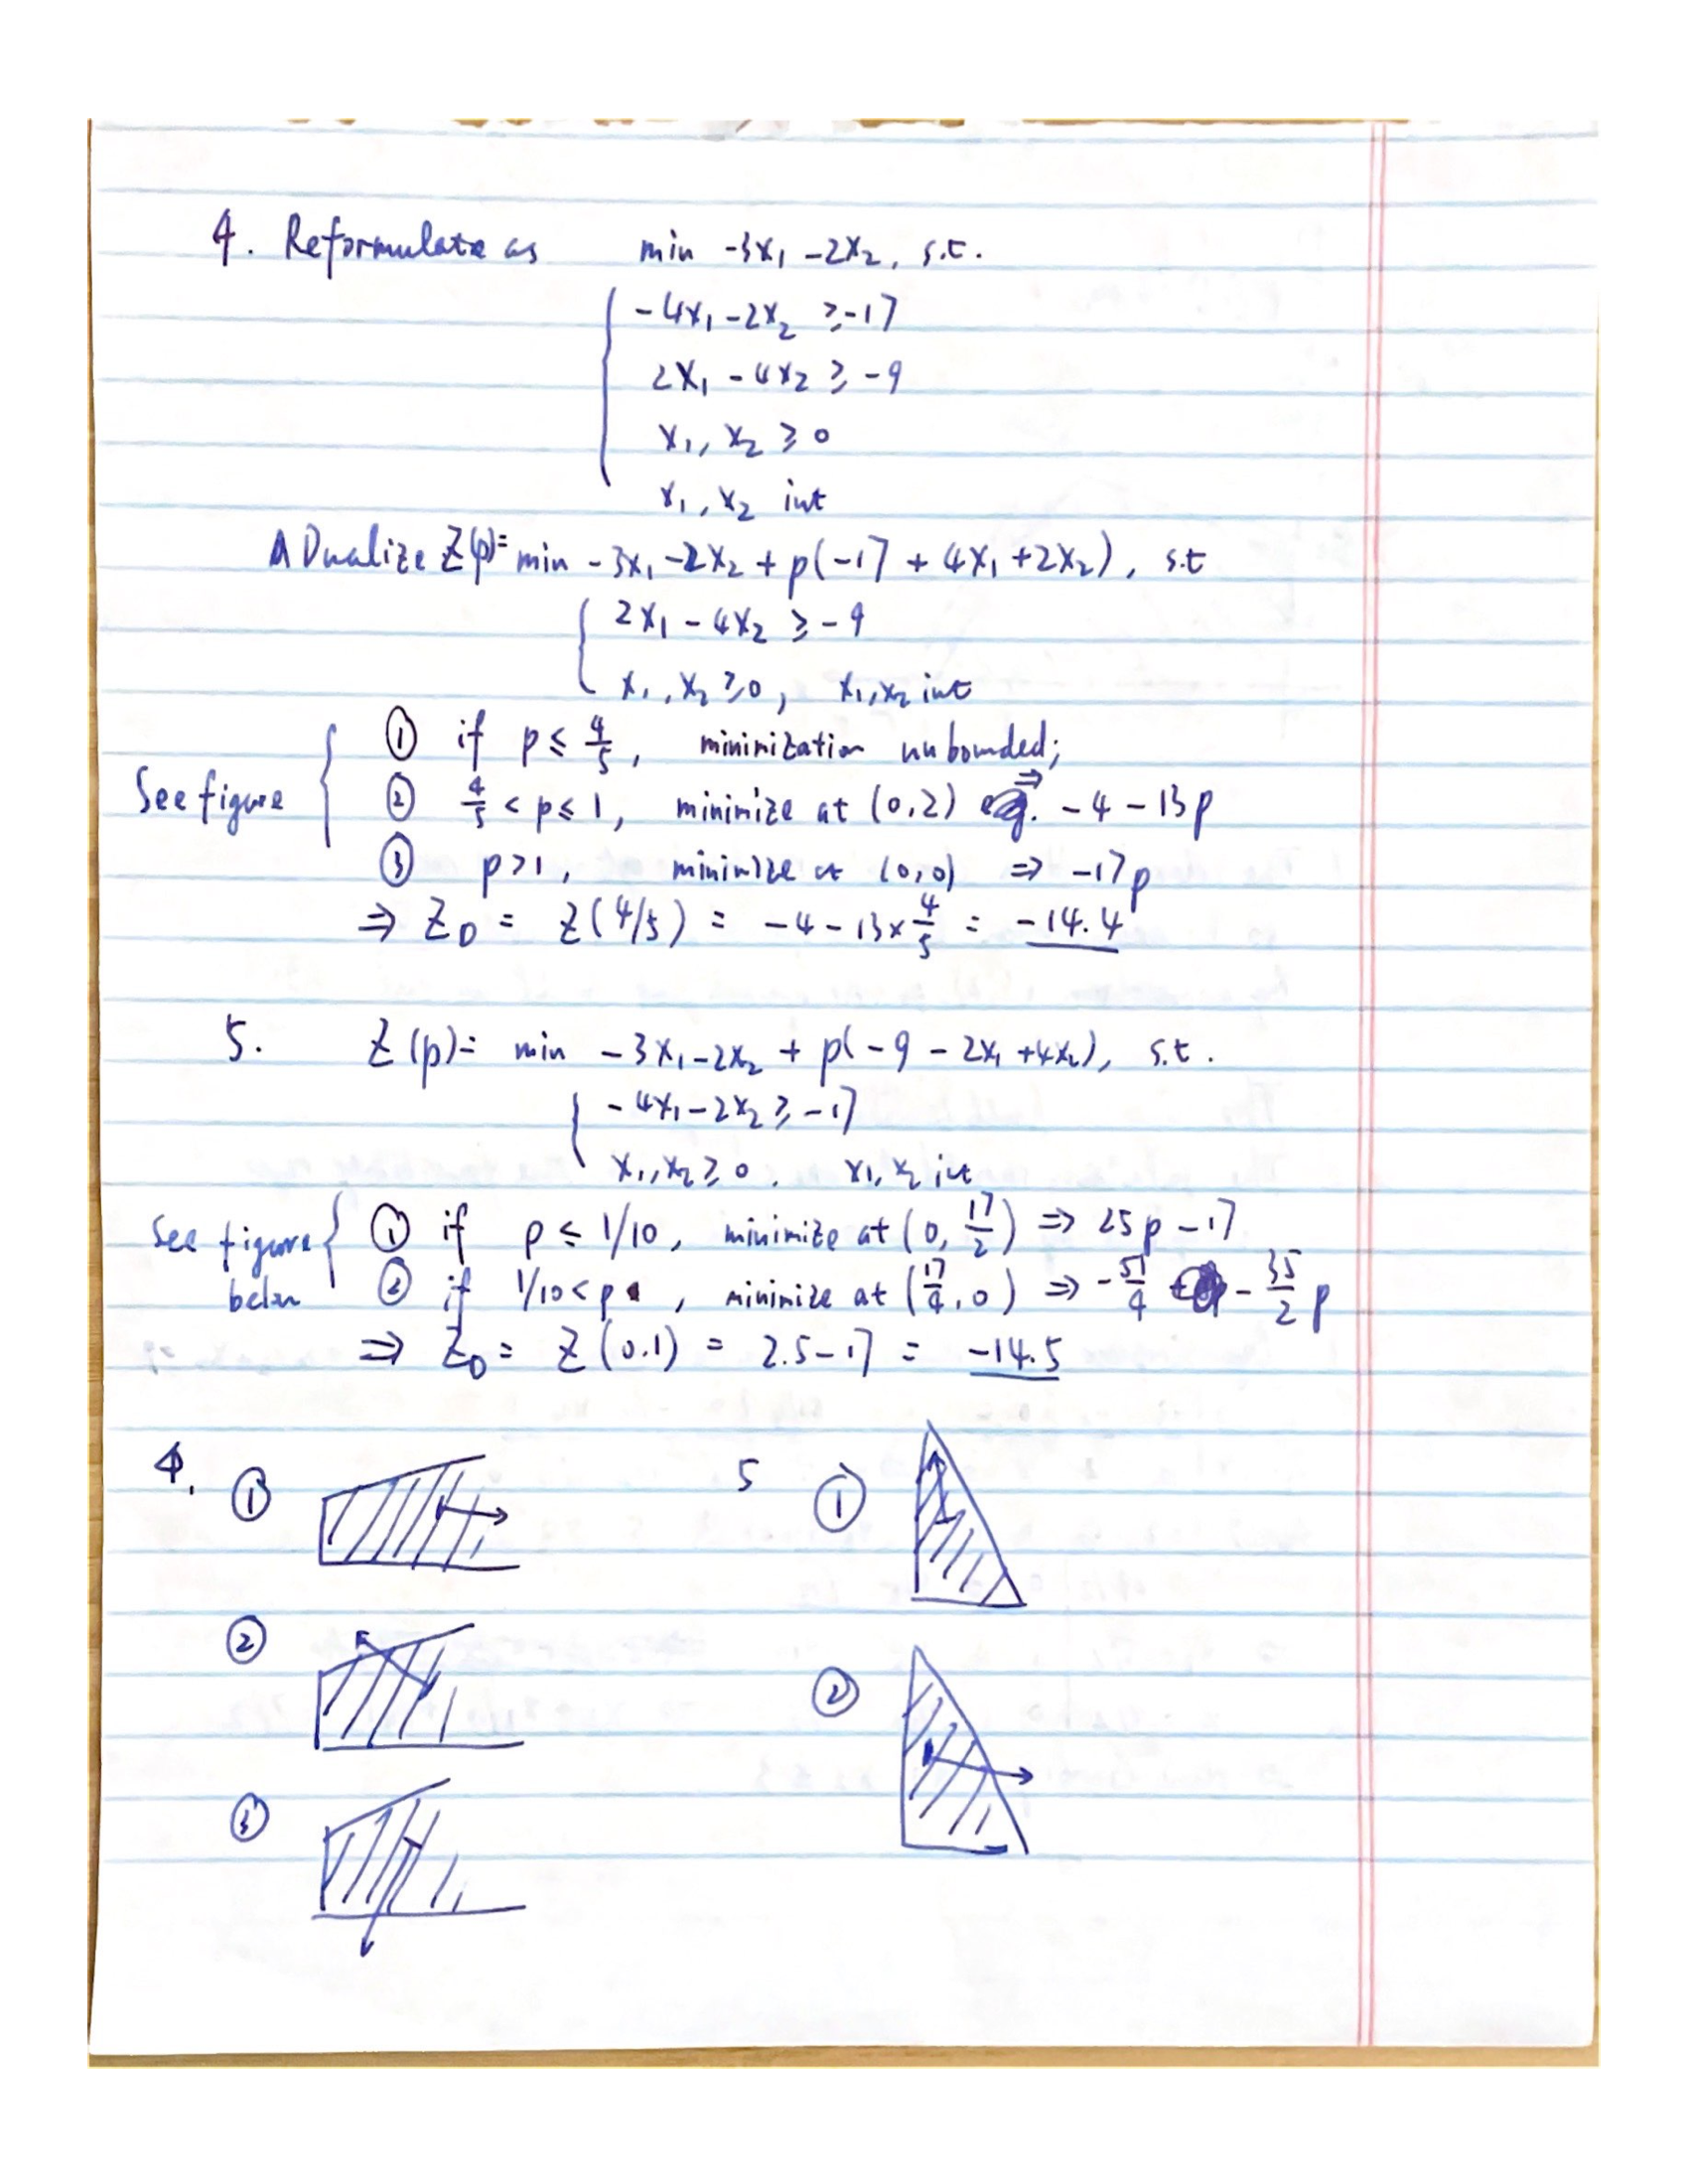
\includegraphics[width=\textwidth]{1.2.png}
    \caption{Solution to Problem 1}
\end{figure}

\section{}
\subsection{}
$$
s_1+ s_2 + s_3 + ... + s_n = 3*i, \quad i \in \mathbb{Z} 
$$ 
i.e, the sum of the set S is divisible by 3.

\subsection{}

Let $f(a, b, c, s)$ be the state with the information that $a, b, c$ represent the remaining sum of integers in each group, while using the first $s$ elements in the set $S$. If this is possible, $f=1$, else $f=0$

The state transition equation would be:

$$
f(a,b,c,s) = f(a-S[s],b,c,s-1) \text{ or } f(a,b-S[s],c,s-1) \text{ or } f(a,b,c-S[s],s-1)
$$

and the base cases would be $f(0,0,0,0)=1$ and $f(a,b,c,0)=0$ if not all $a,b,c$ equals 0.

We can obtain the actual partition method when calculating the state transition: mark the dependence of $f(a,b,c,s)$ with $(s,A)$ if it uses $f(a-S[s],b,c,s-1)$, and similarly for set B and C. We collect all marks toward the final solution and we can get the partition method.


\subsection{}

Let $a_i, b_i, c_i, i= 1, ..., n $ denote to position of each number, if $s_i$ is in the subset A, then $a_i = 1, b_i = 0, c_i = 0$, if in B, $a_i = 0, b_i = 1, c_i = 0$, if C, then $a_i = 0, b_i = 0, c_i = 1$

The integer programming formulation for this problem can be set as:

\begin{align*}
    &\max m\quad \\
    \text{s.t.} \quad& \sum_ia_i\ge m, \sum_ib_i\ge m, \sum_ic_i\ge m  \\
    \quad & \sum_ia_i s_i = \sum_i b_i s_i = \sum_i c_i s_i = \frac{1}{3}\sum_is_i\\
    & a_i+ b_i+ c_i = 1, \quad i = 1, ... n \\
    & a_i, b_i, c_i \in \{0, 1\}
\end{align*}




\section{}
We denote the set defined by the first set, second set and third constraint to be $C_1,C_2,C_3$, and set $0\le x_{ij}\le 1$ to be $C_4$. Denoting the feasible set after four kinds of relaxations to be $X_1=C_1\cap C_2\cap C_4\cap\mathbb Z$, $X_2=C_3\cap C_4\cap\mathbb Z$, $X_3=C_2\cap C_3\cap C_4\cap\mathbb Z$, and $X_4=C_2\cap C_4\cap\mathbb Z$. Let $\x=\{x_{ij}\}$ $z=\sum_{ij}c_{ij}x_{ij}$, we have

\begin{itemize}
    \item $Z_{LP}=\min z$ s.t. $\x\in P_{LP}=C_1\cap C_2\cap C_3\cap C_4$;
    \item $Z_{D1}=\min z$ s.t. $\x\in P_1=C_3\cap \operatorname{CH}(X_1)$;
    \item $Z_{D2}=\min z$ s.t. $\x\in P_2=C_1\cap C_2\cap \operatorname{CH}(X_2)$;
    \item $Z_{D3}=\min z$ s.t. $\x\in P_3=C_1\cap \operatorname{CH}(X_3)$;
    \item $Z_{D4}=\min z$ s.t. $\x\in P_4=C_1\cap C_3\cap \operatorname{CH}(X_4)$;
    \item $Z_{IP}=\min z$ s.t. $\x\in P_{IP}=C_1\cap C_2\cap C_3\cap C_4\cap\mathbb Z$;
\end{itemize}

We first give a lemma on the property of convex hulls: if $A$ is a convex set and $B$ is an arbitrary set, then $\operatorname{CH}(A\cap B)$ is a subset of $A\cap\operatorname{CH}(B)$. This is because for any point in the former set, there exists a convex combination of points in $A\cap B$ that yields this point; and therefore this point is a member of both $\operatorname{CH}(B)$ and $\operatorname{CH}(A)$. Since $A=\operatorname{CH}(A)$, the point is a member of $A\cap\operatorname{CH}(B)$.


Using this lemma, we get $C_1\cap C_2\cap \operatorname{CH}(X_2)\subseteq C_1\cap C_2\cap C_3\cap \operatorname{CH}(C_4\cap\mathbb Z)=C_1\cap C_2\cap C_3\cap C_4$, therefore $P_2\subseteq P_{LP}$, so $Z_{LP}\le Z_{D2}$. Similarly, we can trivially get $Z_{D2}\le Z_{D3}\le Z_{IP}$.

When the third constraint is relaxed, the problem can be reformulated as a network flow problem, and the integrality of such problems implies that solving each subproblem $Z_{D1}(p)$ in $\operatorname{CH}(X_1)$ is equivalent to solving in $C_1\cap C_2\cap C_4$, therefore we have $Z_{D1}=Z_{LP}$. Similarly $Z_{D4}=Z_{LP}$. Assembling all the relationship we got so far gives us the desired order.

\section{}
\subsection{}
\begin{align*}
    \log \mathbb{P}[\Tilde{z_j} = 0] & = \log(\prod_{i \in I^{+}_{j}} \mathbb{P}[\Tilde{y_i} = 0]\prod_{i \in I^{-}_{j}} \mathbb{P}[\Tilde{y_i} = 1]) &\\
    & =  \log(\prod_{i \in I^{+}_{j}} (1-y^{*}_i)\prod_{i \in I^{-}_{j}} y^{*}_i) &\\
    & = \sum_{i \in I^{+}_{j}} \log(1-y^{*}_i) + \sum_{i \in I^{-}_{j}} \log y^{*}_i &\\
    & \leq - \sum_{i \in I^{+}_{j}}y^{*}_i - \sum_{i \in I^{-}_{j}}(1-y^{*}_i) &(logarithm \quad inequality \quad by \quad hint)\\
\end{align*}

\subsection{}

\begin{align*}
    \mathbb{E}[\Tilde{z_j}] & = 0 \times \mathbb{P}[\Tilde{z_j} = 0] + 1 \times \mathbb{P}[\Tilde{z_j} = 1] &\\
    & = \mathbb{P}[\Tilde{z_j} = 1] &\\
    & = 1 - \mathbb{P}[\Tilde{z_j} = 0] &\\
    & =  1 - e^{\log \mathbb{P}[\Tilde{z_j} = 0]} &\\
    & \geq  1 - ({ 1 + (1-\frac{1}{e})\log  \mathbb{P}[\Tilde{z_j} = 0]}) &(logarithm \quad inequality \quad by \quad hint)\\
    & = \frac{e-1}{e}(-\log \mathbb{P}[\Tilde{z_j} = 0])&\\
    & \geq \frac{e-1}{e}( \sum_{i \in I^{+}_{j}}y^{*}_i + \sum_{i \in I^{-}_{j}}(1-y^{*}_i))& (4.1)\\
    & \geq \frac{e-1}{e} z^{*}_{j}
\end{align*}

\subsection{}

\begin{align*}
    Z_{LP} & \geq Z_{IP} & (LP \quad relaxation \quad is \quad an \quad upper-bound \quad of \quad IP)\\
    & \geq \mathbb{E}[Z_H]=\sum_j w_j \mathbb E[\tilde z_{j}] & (\mathbb{E}[Z_H] \leq \max Z_H = Z_{IP})\\
    & \geq \sum_j\frac{e-1}{e} w_jz^{*}_{j} =  \frac{e-1}{e} Z_{LP} & (4.2)\\
\end{align*}

\end{document}
